
\documentclass{beamer}
\mode<presentation>
{
  \usetheme{default}
  \usecolortheme{crane}
  \usefonttheme{structurebold}
  \setbeamertemplate{navigation symbols}{}
  \setbeamertemplate{caption}[numbered]
}

% Single override on top of the crane theme: drop the orange frame-title
% bar AND the orange title-page block. Keep crane's dark text color for
% readability against the white background.
\setbeamercolor{frametitle}{bg=white}
\setbeamercolor{title}{bg=white}

\usepackage[utf8]{inputenc}
\usepackage{fontspec}
\newfontfamily\japanesefont{Noto Sans CJK JP}[Scale=1.0]
\newfontfamily\titlefont{Noto Sans CJK JP Black}[Scale=1.0]
\usepackage{amsmath}
\usepackage{amssymb}
\usepackage{amsthm}
\usepackage{booktabs}
\usepackage{color}
\usepackage{comment}
\usepackage{hyperref}
\usepackage{tikz}
\usetikzlibrary{quantikz}
\usetikzlibrary{shadows.blur, backgrounds, decorations.pathmorphing}
\usetikzlibrary{arrows.meta,positioning,decorations.pathreplacing,calligraphy}

\renewcommand{\>}{\rangle}
\newcommand{\<}{\langle}

\newcommand{\C}{\mathbb{C}}
\newcommand{\F}{\mathbb{F}}
\newcommand{\R}{\mathbb{R}}
\newcommand{\Z}{\mathbb{Z}}

\newcommand{\tr}{\mathrm{tr}}
\newcommand{\Sh}{\mathrm{Sh}}
\newcommand{\Om}{\Omega}
\newcommand{\AOm}{\mathcal{A}_\Omega}
\newcommand{\calP}{\mathcal{P}}
\newcommand{\tA}{\widetilde{A}}

\definecolor{neongreen}{RGB}{0, 255, 128}
\definecolor{neonpink}{RGB}{255, 20, 147}
\definecolor{neonblue}{RGB}{0, 255, 255}
\definecolor{neonyellow}{RGB}{255, 220, 0}
\definecolor{neonorange}{RGB}{255, 110, 50}
\definecolor{neonred}{RGB}{255, 60, 80}
\definecolor{toriired}{RGB}{210, 60, 30}
\definecolor{yamanotegreen}{RGB}{102, 200, 82}
\definecolor{neonpurple}{RGB}{180, 0, 255}
\definecolor{neonmagenta}{RGB}{255, 0, 200}
\definecolor{neongrid}{RGB}{255, 0, 255}
\definecolor{spaceblack}{RGB}{8,4,28}
\definecolor{deepviolet}{RGB}{40,10,80}
\definecolor{fujishadow}{RGB}{60,20,90}
\definecolor{citywindow}{RGB}{255, 230, 100}
\definecolor{gridcolor}{RGB}{255, 109, 194}

%----------------------------------------------------------
%  Reusable TikZ figure components
%----------------------------------------------------------

% Mt. Fuji silhouette: \fujimountain{cx}{cy}{scale}
\newcommand{\fujimountain}[3]{%
  \begin{scope}[shift={(#1, #2)}, scale=#3]
    \fill[fujishadow]
      (-3.2, 0) -- (-1.05, 1.25) 
      .. controls (-0.7, 1.45) and (-0.5, 1.55) .. (-0.4, 1.62)
      .. controls (-0.2, 1.68) and (0.2, 1.68) .. (0.4, 1.62)
      .. controls (0.5, 1.55) and (0.7, 1.45) .. (1.05, 1.25)
      -- (3.2, 0) -- cycle;
    \draw[neonpurple, line width=1.0pt, opacity=0.9]
      (-3.2, 0) -- (-1.05, 1.25) 
      .. controls (-0.7, 1.45) and (-0.5, 1.55) .. (-0.4, 1.62)
      .. controls (-0.2, 1.68) and (0.2, 1.68) .. (0.4, 1.62)
      .. controls (0.5, 1.55) and (0.7, 1.45) .. (1.05, 1.25)
      -- (3.2, 0);
    \fill[white, opacity=0.92]
      (-0.55, 1.32) 
      -- (-0.4, 1.62)
      .. controls (-0.2, 1.68) and (0.2, 1.68) .. (0.4, 1.62)
      -- (0.55, 1.32)
      -- (0.48, 1.36) -- (0.40, 1.30) -- (0.30, 1.38) -- (0.20, 1.31) 
      -- (0.10, 1.38) -- (0.00, 1.30) -- (-0.10, 1.37) -- (-0.20, 1.30) 
      -- (-0.30, 1.38) -- (-0.40, 1.31) -- (-0.48, 1.36) -- cycle;
  \end{scope}
}

% Receding synthwave grid: \synthwavegrid{shift_y}{depth}
\newcommand{\synthwavegrid}[2]{%
  \begin{scope}[shift={(0,#1)}]
    \foreach \i in {0,1,...,20} {
      \pgfmathsetmacro{\xL}{-6 + 0.6*\i}
      \pgfmathsetmacro{\op}{0.3 + 0.5*(\i/20)}
      \draw[neongrid, opacity=\op, thick] (\xL, 0) -- (0, #2);
    }
    \foreach \k in {0,1,...,8} {
      \pgfmathsetmacro{\y}{#2 - #2*(1 - 1/(1 + 0.4*\k))}
      \pgfmathsetmacro{\op}{0.3 + 0.5*(\k/8)}
      \pgfmathsetmacro{\w}{6 - 6*(1 - 1/(1 + 0.4*\k))}
      \draw[neongrid, opacity=\op, thick] (-\w, \y) -- (\w, \y);
    }
  \end{scope}
}

% Pedestrian silhouette: \pedestrian{x}{y}{scale}{color}
\newcommand{\pedestrian}[4]{%
  \begin{scope}[shift={(#1, #2)}, scale=#3]
    \fill[#4] (0, 0.32) circle (0.07);
    \fill[#4] (-0.09, -0.03) -- (-0.075, 0.25) -- (0.075, 0.25) -- (0.09, -0.03) -- cycle;
    \fill[#4] (-0.07, -0.22) rectangle (-0.015, -0.03);
    \fill[#4] (0.015, -0.22) rectangle (0.07, -0.03);
  \end{scope}
}

%%

\title{A Factorization Identity for\\
Twisted Multinomial Coefficients\\
with Application to Pilot States in\\
Hamiltonian Decoded Quantum Interferometry}
\author{Pawe\l{} Wocjan}
\institute{Quantum Algorithms Group, IBM Quantum}
\date{April 28, 2026}

\begin{document}

\begin{frame}
  \titlepage
\end{frame}


%==========================================================
%  Reference
%==========================================================
\begin{frame}{Based on}

    \emph{A Factorization Identity for Twisted Multinomial Coefficients
    with Application to Pilot States in Hamiltonian Decoded Quantum
    Interferometry}

    \medskip
    Pawe\l{} Wocjan, \href{https://arxiv.org/abs/2604.01022}{arXiv:2604.01022} (April 2026)

    \bigskip\bigskip
    Builds on:

    \medskip
    \begin{itemize}
        \item A.~Schmidhuber, J.~Lu, N.~Shutty, S.~Jordan, A.~Poremba, Y.~Quek, \emph{Hamiltonian Decoded Quantum Interferometry},
        arXiv:2510.07913.

        \medskip
        \item K.~Bu, W.~Gu, X.~Li, \emph{Hamiltonian decoded quantum interferometry for general Pauli Hamiltonians}, arXiv:2601.18773.
    \end{itemize}
\end{frame}

%==========================================================
%  ENKEI -- distant view (overview)
%==========================================================

\begin{frame}{遠景 Enkei -- Distant View}

\begin{center}
\begin{tikzpicture}[scale=0.95, background rectangle/.style={fill=spaceblack}, show background rectangle]

% Stars
\foreach \i in {1,...,180} {
  \pgfmathsetmacro{\x}{rnd*12 - 6}
  \pgfmathsetmacro{\y}{rnd*3.2 + 0.6}
  \pgfmathsetmacro{\s}{0.008 + rnd*0.022}
  \pgfmathsetmacro{\op}{0.3 + rnd*0.6}
  \fill[white, opacity=\op] (\x,\y) circle (\s);
}

% Synthwave sun
\begin{scope}
  \clip (-3,0) rectangle (3, 3);
  \shade[inner color=neonyellow, outer color=neonpink] (0,0) circle (2.4);
\end{scope}
\foreach \y in {0.18, 0.55, 0.95, 1.4, 1.9} {
  \pgfmathsetmacro{\h}{0.06 + 0.012*\y}
  \fill[spaceblack] (-3, \y - \h) rectangle (3, \y + \h);
}

% Mt. Fuji
\fujimountain{0}{0}{1.0}

% Grid
\synthwavegrid{-2.6}{2.6}

% Titles
\node[neonpink] at (0, 3.7) {\Large {\japanesefont 遠景}};

\end{tikzpicture}
\end{center}
\end{frame}

%%

\begin{frame}{Enkei Summary I -- HDQI}

\begin{itemize}
    \item \textbf{Hamiltonian Decoded Quantum Interferometry} (Schmidhuber
    et al.~2025): a quantum algorithm that
    prepares Gibbs and ground states of many-body Hamiltonians.

    \bigskip
    \item Inside HDQI, the central data is a so-called \textbf{pilot state}.
\end{itemize}
\end{frame}

%%

\begin{frame}{HDQI -- the protocol in three steps}

\bigskip
\begin{center}
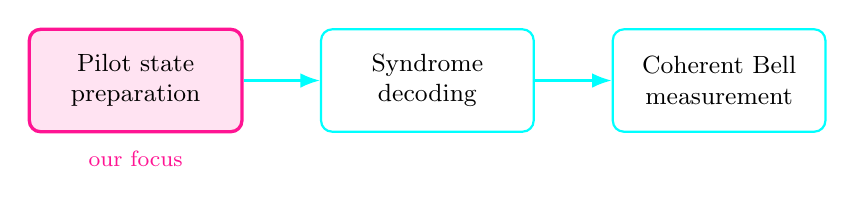
\begin{tikzpicture}[scale=0.95,
    box/.style={rectangle, rounded corners=4pt, draw=neonblue, minimum width=2.7cm, minimum height=1.3cm, thick, align=center, inner sep=3pt, font=\small},
    ours/.style={rectangle, rounded corners=4pt, draw=neonpink, fill=neonpink!12, minimum width=2.7cm, minimum height=1.3cm, very thick, align=center, inner sep=3pt, font=\small},
    arrow/.style={-{Latex[length=2.5mm]}, thick, neonblue}]

\node[ours] (pilot) at (0, 0) {Pilot state\\preparation};
\node[box] (decode) at (3.9, 0) {Syndrome\\decoding};
\node[box] (bell) at (7.8, 0) {Coherent Bell\\measurement};

\draw[arrow] (pilot) -- (decode);
\draw[arrow] (decode) -- (bell);

\node[neonpink, font=\footnotesize] at (0, -1.05) {our focus};

\end{tikzpicture}
\end{center}

\bigskip
\begin{itemize}
    \item We address only the \emph{first} step.
    \medskip
    \item Decoding is a separate problem; both must work together for HDQI to succeed.
\end{itemize}
\end{frame}

%%

\begin{frame}{Enkei Summary II -- the bottleneck}

\begin{itemize}
    \item For an $n$-qubit Pauli Hamiltonian 
    \begin{align*}
        H = \sum_{j=1}^m c_j P_j,
    \end{align*}    
    the pilot state encodes the coefficients of $H^k$ in the Pauli basis:
    
    \begin{align*}
        H^k = \sum_{r\in\{0,1\}^m} \alpha_r \, P_1^{r_1}\cdots P_m^{r_m}.
    \end{align*}
    
    \bigskip
    \item There are $2^m$ amplitudes -- exponentially many.

    \bigskip
    \item \emph{Computing them efficiently is the bottleneck.}
\end{itemize}
\end{frame}

%%

\begin{frame}{Enkei Summary III -- our contribution}

\begin{itemize}
    \item We identify a structural condition on the Pauli commutation
    pattern -- \textbf{predecessor-uniformity} -- that yields:

    \medskip
    \begin{itemize}
        \item a clean \textbf{combinatorial identity} for so-called
        \emph{twisted multinomial coefficients}, generalizing the
        classical $q$-multinomial,

        \medskip
        \item an \textbf{exact MPS of bond dimension $k+1$} for the
        pilot state amplitudes.
    \end{itemize}

    \bigskip
    \item For mutually anticommuting generators, this is an
    \emph{exponential improvement} over previous methods.
\end{itemize}
\end{frame}


\begin{frame}{中景 Chūkei -- Middle View}
\begin{center}
\begin{tikzpicture}[scale=0.95, background rectangle/.style={fill=spaceblack}, show background rectangle]

% Stars
\foreach \i in {1,...,100} {
  \pgfmathsetmacro{\x}{rnd*12 - 6}
  \pgfmathsetmacro{\y}{rnd*2.5 + 1.2}
  \pgfmathsetmacro{\s}{0.008 + rnd*0.018}
  \pgfmathsetmacro{\op}{0.25 + rnd*0.55}
  \fill[white, opacity=\op] (\x,\y) circle (\s);
}

% Synthwave sun behind Fuji
\begin{scope}
  \clip (-3.0, 0) rectangle (3.0, 3.0);
  \shade[inner color=neonyellow, outer color=neonpink] (0, 0) circle (2.6);
\end{scope}
% Horizontal stripes across the sun
\foreach \y in {0.18, 0.55, 0.95, 1.4, 1.9} {
  \pgfmathsetmacro{\h}{0.06 + 0.012*\y}
  \fill[spaceblack] (-3, \y - \h) rectangle (3, \y + \h);
}

% Receding grid -- drawn BEFORE foreground so buildings/Shinkansen sit ON TOP of it
\synthwavegrid{-2.6}{2.6}

% Mt. Fuji (slightly left, slightly bigger; base anchored on the grid horizon at y=0)
\fujimountain{-0.5}{0}{1.45}

%====== FOREGROUND BUILDINGS (closer than Fuji) ======
% Drawn AFTER Fuji so they overlap Fuji's lower slopes -- this is the depth cue.
% Bases below horizon (y < 0), tops up around y ~ 1.0-1.5.

% Left cluster
% LB1 -- closer/taller, leftmost
\fill[fujishadow!90] (-5.6, -1.3) rectangle (-4.6, 1.4);
\draw[neonblue, line width=0.8pt] (-5.6, -1.3) rectangle (-4.6, 1.4);
\foreach \y in {-1.0, -0.6, -0.2, 0.2, 0.6, 1.0} {
  \foreach \x in {-5.45, -5.15, -4.85} {
    \pgfmathsetmacro{\op}{0.25 + rnd*0.45}
    \fill[neonblue, opacity=\op] (\x, \y) rectangle ++(0.10, 0.13);
  }
}
% LB2 -- shorter, to its right (overlaps Fuji's lower slope)
\fill[fujishadow!90] (-4.55, -1.3) rectangle (-3.85, 0.6);
\draw[neonpurple, line width=0.8pt] (-4.55, -1.3) rectangle (-3.85, 0.6);
\foreach \y in {-1.0, -0.6, -0.2, 0.2} {
  \foreach \x in {-4.40, -4.18, -3.96} {
    \pgfmathsetmacro{\op}{0.25 + rnd*0.45}
    \fill[neonpurple, opacity=\op] (\x, \y) rectangle ++(0.08, 0.11);
  }
}

% Right cluster
% RB1 -- right of Tokyo Tower position
\fill[fujishadow!90] (5.20, -1.3) rectangle (5.95, 0.9);
\draw[neonpink, line width=0.8pt] (5.20, -1.3) rectangle (5.95, 0.9);
\foreach \y in {-1.0, -0.6, -0.2, 0.2, 0.6} {
  \foreach \x in {5.30, 5.55, 5.78} {
    \pgfmathsetmacro{\op}{0.25 + rnd*0.45}
    \fill[neonpink, opacity=\op] (\x, \y) rectangle ++(0.10, 0.13);
  }
}

%====== TOKYO TOWER -- redesigned as visible lattice ======
\begin{scope}[shift={(4.4, -0.3)}, scale=1.3]
  \draw[neonred, line width=1.4pt]
    (-0.55, 0)
    -- (-0.40, 0.40) -- (-0.32, 0.85)
    -- (-0.42, 0.95) -- (-0.42, 1.10)
    -- (-0.27, 1.20) -- (-0.18, 1.55) -- (-0.13, 1.80)
    -- (-0.20, 1.85) -- (-0.20, 1.97)
    -- (-0.10, 2.05) -- (-0.05, 2.30) -- (-0.03, 2.50)
    -- (0.03, 2.50) -- (0.05, 2.30) -- (0.10, 2.05)
    -- (0.20, 1.97) -- (0.20, 1.85) -- (0.13, 1.80)
    -- (0.18, 1.55) -- (0.27, 1.20)
    -- (0.42, 1.10) -- (0.42, 0.95)
    -- (0.32, 0.85) -- (0.40, 0.40) -- (0.55, 0)
    -- cycle;

  \draw[neonred, opacity=0.7, line width=0.6pt] (-0.55, 0) -- (-0.32, 0.85);
  \draw[neonred, opacity=0.7, line width=0.6pt] (0.55, 0) -- (0.32, 0.85);
  \foreach \k in {0,1,2} {
    \pgfmathsetmacro{\yL}{0 + 0.283*\k}
    \pgfmathsetmacro{\yU}{0.283*(\k+1)}
    \pgfmathsetmacro{\xLL}{-0.55 + 0.27*\k/3}
    \pgfmathsetmacro{\xLR}{0.55 - 0.27*\k/3}
    \pgfmathsetmacro{\xUL}{-0.55 + 0.27*(\k+1)/3}
    \pgfmathsetmacro{\xUR}{0.55 - 0.27*(\k+1)/3}
    \draw[neonred, opacity=0.6, line width=0.4pt] (\xLL, \yL) -- (\xUR, \yU);
    \draw[neonred, opacity=0.6, line width=0.4pt] (\xLR, \yL) -- (\xUL, \yU);
    \draw[neonred, opacity=0.5, line width=0.4pt] (\xUL, \yU) -- (\xUR, \yU);
  }

  \fill[neonred, opacity=0.85] (-0.42, 0.95) rectangle (0.42, 1.10);
  \draw[neonred, line width=0.8pt] (-0.42, 0.95) rectangle (0.42, 1.10);

  \draw[neonred, opacity=0.7, line width=0.5pt] (-0.27, 1.20) -- (-0.13, 1.80);
  \draw[neonred, opacity=0.7, line width=0.5pt] (0.27, 1.20) -- (0.13, 1.80);
  \foreach \k in {0,1} {
    \pgfmathsetmacro{\yL}{1.20 + 0.30*\k}
    \pgfmathsetmacro{\yU}{1.20 + 0.30*(\k+1)}
    \pgfmathsetmacro{\xLL}{-0.27 + 0.14*\k/2}
    \pgfmathsetmacro{\xLR}{0.27 - 0.14*\k/2}
    \pgfmathsetmacro{\xUL}{-0.27 + 0.14*(\k+1)/2}
    \pgfmathsetmacro{\xUR}{0.27 - 0.14*(\k+1)/2}
    \draw[neonred, opacity=0.55, line width=0.35pt] (\xLL, \yL) -- (\xUR, \yU);
    \draw[neonred, opacity=0.55, line width=0.35pt] (\xLR, \yL) -- (\xUL, \yU);
    \draw[neonred, opacity=0.45, line width=0.35pt] (\xUL, \yU) -- (\xUR, \yU);
  }

  \fill[neonred, opacity=0.85] (-0.20, 1.85) rectangle (0.20, 1.97);
  \draw[neonred, line width=0.7pt] (-0.20, 1.85) rectangle (0.20, 1.97);

  \draw[neonred, opacity=0.6, line width=0.4pt] (-0.10, 2.05) -- (-0.03, 2.50);
  \draw[neonred, opacity=0.6, line width=0.4pt] (0.10, 2.05) -- (0.03, 2.50);

  \draw[neonred, line width=1.0pt] (0, 2.50) -- (0, 3.10);
  \fill[neonyellow] (0, 3.10) circle (0.045);
  \fill[neonyellow!80] (0, 2.85) circle (0.025);
\end{scope}

% Shinkansen streak straddling the horizon line at y=0
\begin{scope}
  \shade[left color=spaceblack, right color=neonblue] (-2.8, -0.05) rectangle (-0.5, 0.10);
  \fill[neonblue] (-0.5, -0.05) -- (-0.1, 0.025) -- (-0.5, 0.10) -- cycle;
  \fill[neonblue, opacity=0.30] (-3.2, -0.15) rectangle (-0.1, 0.20);
\end{scope}

\node[neonpink] at (0, 3.7) {\Large {\japanesefont 中景}};

\end{tikzpicture}
\end{center}
\end{frame}


%%

\begin{frame}{A familiar object -- the multinomial coefficient}

\begin{itemize}
    \item $\binom{k}{k_1,\ldots,k_m}$ counts arrangements of the multiset
    $\{1^{k_1},\ldots,m^{k_m}\}$.

    \bigskip
    \item \textit{Example.} $\binom{3}{2,1} = 3$ arrangements of two
    $1$'s and one $2$:
    \begin{align*}
        1\,1\,2 \qquad 1\,2\,1 \qquad 2\,1\,1
    \end{align*}
\end{itemize}
\end{frame}

%%

\begin{frame}{Refining by inversions -- the $q$-multinomial}

\begin{itemize}
    \item Weight each arrangement by $q^{\#\mathrm{inversions}}$, where an
    \emph{inversion} is a pair of positions where a larger letter
    precedes a smaller one.

    \bigskip
    \item \textit{Same example.}
    \begin{align*}
        1\,1\,2 \quad &\to \quad 0 \text{ inversions} \quad\to\quad 1 \\[2pt]
        1\,2\,1 \quad &\to \quad 1 \text{ inversion} \quad\to\quad q \\[2pt]
        2\,1\,1 \quad &\to \quad 2 \text{ inversions} \quad\to\quad q^2
    \end{align*}

    \medskip
    \item Sum: $\;\binom{3}{2,1}_q = 1 + q + q^2$.
\end{itemize}
\end{frame}

%%

\begin{frame}{The classical factorization}

\begin{itemize}
    \item The $q$-multinomial factors as a product of \emph{Gaussian
    binomials}:
    \begin{align*}
        \binom{k}{k_1,\ldots,k_m}_q
        \;=\;
        \prod_{j=1}^m \binom{\ell_j}{k_j}_q,
        \qquad
        \ell_j = k_1 + \cdots + k_j.
    \end{align*}

    \bigskip
    \item Picture: build any arrangement \textbf{one letter type at a
    time}, interleaving the $k_j$ copies of letter $j$ into the existing word.

    \medskip
    Each stage contributes one Gaussian binomial.
\end{itemize}
\end{frame}

%%

\begin{frame}{The new object -- twisted multinomial}

\begin{itemize}
    \item In the $q$-multinomial, every inversion has the \emph{same}
    weight $q$.

    \bigskip
    \item \textbf{Twisted version.} Each inversion of types $i<j$ carries
    its own weight $\omega_{ij}$:
    \begin{align*}
        \binom{k}{k_1,\dots,k_m}_\Omega
        \;:=\!
        \sum_{\sigma}\;\;
        \prod_{\substack{\text{inversions}\\\text{of type }(i,j)}}
        \omega_{ij}.
    \end{align*}

    \bigskip
    \item Specializing $\omega_{ij}\equiv q$ recovers the $q$-multinomial.

    \medskip
    \item In general: \emph{no clean factorization.}
\end{itemize}
\end{frame}

%%

\begin{frame}{Concrete example -- $\binom{3}{1,1,1}_\Omega$}

Six arrangements of $\{1,2,3\}$, each with its inversion weight:

\medskip
\begin{center}
\begin{tabular}{c@{\quad}c}
\toprule
arrangement & weight \\
\midrule
$1\,2\,3$ & $1$ \\
$1\,3\,2$ & $\omega_{2,3}$ \\
$2\,1\,3$ & $\omega_{1,2}$ \\
$2\,3\,1$ & $\omega_{1,2}\,\omega_{1,3}$ \\
$3\,1\,2$ & $\omega_{1,3}\,\omega_{2,3}$ \\
$3\,2\,1$ & $\omega_{1,2}\,\omega_{1,3}\,\omega_{2,3}$ \\
\bottomrule
\end{tabular}
\end{center}

\medskip
\begin{align*}
\binom{3}{1,1,1}_\Omega 
&=
1 + \omega_{1,2} + \omega_{2,3} + \omega_{1,2}\omega_{1,3} 
+ \omega_{1,3}\omega_{2,3} + \omega_{1,2}\omega_{1,3}\omega_{2,3}.
\end{align*}

\end{frame}

%%

\begin{frame}{What makes the twisted multinomial factor?}

\begin{itemize}
    \item In the classical proof, all stages of the build-up
    contribute the \emph{same} weight $q$, so they decouple.

    \bigskip
    \item In the twisted case, the weight of inserting a letter $j$
    depends on \emph{which} earlier letters it crosses.

    \bigskip
    \item We need a structural condition to make stages decouple again.

    \bigskip
    \item Enter \emph{predecessor-uniformity}.
\end{itemize}
\end{frame}

%%

\begin{frame}{Predecessor-uniformity -- the picture}

\begin{center}
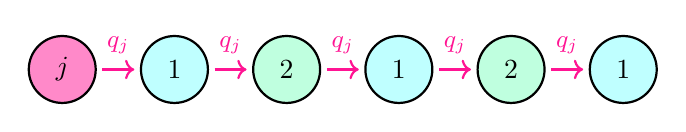
\begin{tikzpicture}[scale=0.95,
    letter/.style={circle, draw, minimum size=0.85cm, thick}]

% The new letter j on the far left
\node[letter, fill=neonpink!50] (b)  at (-1.5, 0) {$j$};

% Existing word: 1 2 1 2 1
\node[letter, fill=neonblue!25]  (a1) at (0,   0) {1};
\node[letter, fill=neongreen!25] (a2) at (1.5, 0) {2};
\node[letter, fill=neonblue!25]  (a3) at (3.0, 0) {1};
\node[letter, fill=neongreen!25] (a4) at (4.5, 0) {2};
\node[letter, fill=neonblue!25]  (a5) at (6.0, 0) {1};

% Five short arrows -- one in each gap between consecutive circles.
% Arrow tips land in the gap (not touching either circle).
% Each labeled q_j to emphasize that the cost is the SAME for every crossing.
\foreach \src/\dst in {b/a1, a1/a2, a2/a3, a3/a4, a4/a5} {
  \draw[->, thick, neonpink, shorten <=2pt, shorten >=2pt] (\src) -- (\dst)
    node[midway, above=2pt] {\small $q_j$};
}

\end{tikzpicture}
\end{center}

\bigskip
\textbf{Predecessor-uniform:} when letter~$j$ crosses any earlier letter
$i<j$, the cost is the \emph{same} $q_j$ -- regardless of which earlier
letter type it is.

\medskip
Formally: $\;\omega_{ij} = q_j\;$ for all $\;i < j$.

\medskip
\emph{Whether $\Omega$ admits a predecessor-uniform ordering is decidable greedily in $O(m^3)$.}
\end{frame}

%%

\begin{frame}{Main theorem}

\textbf{Proposition.}
\emph{If $\Omega$ is predecessor-uniform with parameters $q_2, q_3, \ldots, q_m$, then}
\begin{align*}
    \binom{k}{k_1,\dots,k_m}_\Omega
    \;=\;
    \prod_{j=1}^m \binom{\ell_j}{k_j}_{q_j},
    \qquad
    \ell_j = k_1+\cdots+k_j.
\end{align*}

\bigskip\bigskip
\begin{itemize}
    \item Same shape as the classical product formula.

    \medskip
    \item One $q$ becomes $m{-}1$ \emph{independent} parameters $q_j$
    -- each Gaussian binomial uses its own $q_j$.

    \medskip
    \item Holds for arbitrary $q_j\in\C\setminus\{0\}$ -- no algebraic
    constraint required.
\end{itemize}
\end{frame}

%%

\begin{frame}{Verifying on the example}

For $\binom{3}{1,1,1}_\Omega$ under predecessor-uniformity:
\begin{align*}
    \;\omega_{1,2} = q_2, \;\;\omega_{1,3} = \omega_{2,3} = q_3
\end{align*}

\medskip
Substituting into each arrangement's weight:

\smallskip
\begin{center}
\begin{tabular}{c@{\;\;}c@{\qquad\qquad}c@{\;\;}c}
\toprule
arrangement & weight & arrangement & weight \\
\midrule
$1\,2\,3$ & $1$    & $2\,3\,1$ & $q_2\,q_3$    \\
$1\,3\,2$ & $q_3$  & $3\,1\,2$ & $q_3^2$       \\
$2\,1\,3$ & $q_2$  & $3\,2\,1$ & $q_2\,q_3^2$  \\
\bottomrule
\end{tabular}
\end{center}

\medskip
\begin{align*}
\binom{3}{1,1,1}_\Omega 
&= 1 + q_2 + q_3 + q_2 q_3 + q_3^2 + q_2 q_3^2 \\
&= (1 + q_2)(1 + q_3 + q_3^2) 
\;=\; \binom{2}{1}_{q_2}\binom{3}{1}_{q_3} \quad\checkmark
\end{align*}

\end{frame}
%%

\begin{frame}{The proof in one picture}

At stage $j$, the $u$-th inserted copy of $j$ skips $t_u$ earlier letters. The $t_u$'s form a partition $\lambda$ in a $k_j \times \ell_{j-1}$ box; each skip contributes $q_j$.

\bigskip
\begin{center}
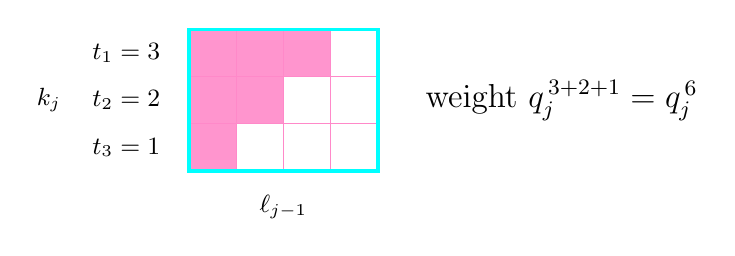
\begin{tikzpicture}[scale=0.6]

% Empty box outline first
\foreach \i in {0,...,3} {
  \foreach \j in {0,...,2} {
    \draw[neonpink!50, thin] (\i, \j) rectangle (\i+1, \j+1);
  }
}

% Partition (3, 2, 1) shaded
\fill[neonpink, opacity=0.45] (0, 2) rectangle (3, 3);
\fill[neonpink, opacity=0.45] (0, 1) rectangle (2, 2);
\fill[neonpink, opacity=0.45] (0, 0) rectangle (1, 1);

% Re-draw grid lines on top
\foreach \i in {0,...,3} {
  \foreach \j in {0,...,2} {
    \draw[neonpink!50, thin] (\i, \j) rectangle (\i+1, \j+1);
  }
}

% Outer box bold
\draw[neonblue, very thick] (0, 0) rectangle (4, 3);

% Row labels (t_1, t_2, t_3) just inside the left edge
\node[right, font=\small] at (-2.25, 2.5) {$t_1=3$};
\node[right, font=\small] at (-2.25, 1.5) {$t_2=2$};
\node[right, font=\small] at (-2.25, 0.5) {$t_3=1$};

% Side annotations
\node[left, font=\small] at (-2.5, 1.5) {$k_j$};
\node[below, font=\small] at (2, -0.3) {$\ell_{j-1}$};

\node[right, font=\large] at (4.8, 1.5) {weight $q_j^{\,3+2+1} = q_j^{\,6}$};

\end{tikzpicture}
\end{center}

\bigskip
\begin{itemize}
    \item Sum over $\lambda$:
    $\;\;\displaystyle\sum_{\lambda \subseteq k_j \times \ell_{j-1}} q_j^{|\lambda|}
    \;=\; \binom{\ell_j}{k_j}_{q_j}.$

    \medskip
    \item Predecessor-uniformity decouples the stages $\Rightarrow$ product formula. \qed
\end{itemize}

\end{frame}

%%

\begin{frame}{近景 Kinkei -- Close-up View}
\hspace*{-0.9cm}\begin{tikzpicture}[scale=0.9, background rectangle/.style={fill=spaceblack}, show background rectangle]

% Stars
\foreach \i in {1,...,40} {
  \pgfmathsetmacro{\x}{rnd*12 - 6}
  \pgfmathsetmacro{\y}{rnd*1.8 + 1.6}
  \pgfmathsetmacro{\s}{0.005 + rnd*0.012}
  \pgfmathsetmacro{\op}{0.2 + rnd*0.4}
  \fill[white, opacity=\op] (\x,\y) circle (\s);
}

% Synthwave sun above horizon
\begin{scope}
  \clip (-0.85, 1.0) rectangle (0.85, 1.95);
  \shade[inner color=neonyellow, outer color=neonpink] (0, 1.0) circle (0.85);
\end{scope}
\fill[spaceblack] (-0.85, 1.20) rectangle (0.85, 1.26);
\fill[spaceblack] (-0.85, 1.46) rectangle (0.85, 1.52);
\fill[spaceblack] (-0.85, 1.74) rectangle (0.85, 1.80);

% Distant Mt. Fuji on horizon
\fill[fujishadow, opacity=0.85]
  (-0.65, 1.0) -- (-0.20, 1.55)
  .. controls (-0.07, 1.62) and (0.07, 1.62) .. (0.20, 1.55)
  -- (0.65, 1.0) -- cycle;
\fill[white, opacity=0.5]
  (-0.20, 1.55) .. controls (-0.07, 1.62) and (0.07, 1.62) .. (0.20, 1.55)
  -- (0.13, 1.50) -- (0.05, 1.55) -- (-0.05, 1.50) -- (-0.13, 1.55) -- cycle;

% Receding street grid
\begin{scope}
  \foreach \i in {0,1,...,10} {
    \pgfmathsetmacro{\xL}{-2.0 + 0.4*\i}
    \pgfmathsetmacro{\op}{0.45 + 0.45*(\i/10)}
    \draw[neongrid, opacity=\op, thick] (\xL, -2.0) -- (0, 1.0);
  }
  \foreach \k in {0,1,...,7} {
    \pgfmathsetmacro{\y}{-2.0 + 3.0*(1 - 1/(1 + 0.5*\k))}
    \pgfmathsetmacro{\op}{0.45 + 0.45*(\k/7)}
    \pgfmathsetmacro{\w}{2.0 - 2.0*(1 - 1/(1 + 0.5*\k))}
    \draw[neongrid, opacity=\op, thick] (-\w, \y) -- (\w, \y);
  }
\end{scope}

% FULL-WIDTH HORIZON LINE at y=1.0
\draw[neonblue, line width=4pt, opacity=0.18] (-6.7, 1.0) -- (6.7, 1.0);
\draw[neonblue, line width=1.4pt, opacity=0.95] (-6.7, 1.0) -- (6.7, 1.0);

%====== BUILDINGS: drawn FAR-to-NEAR, wider, closer to road ======

% L4 (FARTHEST left)
\fill[fujishadow] (-3.0, 0.10) rectangle (-1.85, 0.70);
\draw[neonmagenta, line width=1.0pt] (-3.0, 0.10) rectangle (-1.85, 0.70);
\foreach \y in {0.20, 0.45} {
  \foreach \x in {-2.90, -2.65, -2.40, -2.15, -1.95} {
    \pgfmathsetmacro{\op}{0.25 + rnd*0.55}
    \fill[neonmagenta, opacity=\op] (\x, \y) rectangle ++(0.08, 0.12);
  }
}

% R4 (FARTHEST right)
\fill[fujishadow] (1.85, 0.10) rectangle (3.0, 0.70);
\draw[neonyellow, line width=1.0pt] (1.85, 0.10) rectangle (3.0, 0.70);
\foreach \y in {0.20, 0.45} {
  \foreach \x in {1.95, 2.15, 2.40, 2.65, 2.90} {
    \pgfmathsetmacro{\op}{0.25 + rnd*0.55}
    \fill[neonyellow, opacity=\op] (\x, \y) rectangle ++(0.08, 0.12);
  }
}

% L3
\fill[fujishadow] (-4.10, -0.5) rectangle (-2.85, 1.10);
\draw[neonpurple, line width=1.0pt] (-4.10, -0.5) rectangle (-2.85, 1.10);
\foreach \y in {-0.2, 0.2, 0.6} {
  \foreach \x in {-3.95, -3.65, -3.35, -3.05} {
    \pgfmathsetmacro{\op}{0.25 + rnd*0.65}
    \fill[neonpurple, opacity=\op] (\x, \y) rectangle ++(0.10, 0.15);
  }
}

% R3
\fill[fujishadow] (2.85, -0.5) rectangle (4.10, 1.10);
\draw[neonpink, line width=1.0pt] (2.85, -0.5) rectangle (4.10, 1.10);
\foreach \y in {-0.2, 0.2, 0.6} {
  \foreach \x in {2.95, 3.25, 3.55, 3.85} {
    \pgfmathsetmacro{\op}{0.25 + rnd*0.65}
    \fill[neonpink, opacity=\op] (\x, \y) rectangle ++(0.10, 0.15);
  }
}

% L2
\fill[fujishadow] (-4.90, -1.4) rectangle (-3.70, 2.0);
\draw[neonblue, line width=1.0pt] (-4.90, -1.4) rectangle (-3.70, 2.0);
\foreach \y in {-1.0, -0.5, 0.0, 0.5, 1.0, 1.5} {
  \foreach \x in {-4.75, -4.45, -4.15, -3.85} {
    \pgfmathsetmacro{\op}{0.25 + rnd*0.7}
    \fill[neonblue, opacity=\op] (\x, \y) rectangle ++(0.12, 0.18);
  }
}

% R2
\fill[fujishadow] (3.70, -1.4) rectangle (4.90, 2.0);
\draw[neonorange, line width=1.0pt] (3.70, -1.4) rectangle (4.90, 2.0);
\foreach \y in {-1.0, -0.5, 0.0, 0.5, 1.0, 1.5} {
  \foreach \x in {3.85, 4.15, 4.45, 4.75} {
    \pgfmathsetmacro{\op}{0.25 + rnd*0.7}
    \fill[neonorange, opacity=\op] (\x, \y) rectangle ++(0.12, 0.18);
  }
}

% L1
\fill[fujishadow] (-6.10, -2.0) rectangle (-4.80, 2.85);
\draw[neonpink, line width=1.0pt] (-6.10, -2.0) rectangle (-4.80, 2.85);
\foreach \y in {-1.6, -1.1, -0.6, -0.1, 0.4, 0.9, 1.4, 1.9, 2.4} {
  \foreach \x in {-5.95, -5.65, -5.35, -5.05} {
    \pgfmathsetmacro{\op}{0.25 + rnd*0.7}
    \fill[citywindow, opacity=\op] (\x, \y) rectangle ++(0.13, 0.20);
  }
}

% R1
\fill[fujishadow] (4.80, -2.0) rectangle (6.10, 2.95);
\draw[neonblue, line width=1.0pt] (4.80, -2.0) rectangle (6.10, 2.95);
\foreach \y in {-1.6, -1.1, -0.6, -0.1, 0.4, 0.9, 1.4, 1.9, 2.4} {
  \foreach \x in {4.95, 5.25, 5.55, 5.85} {
    \pgfmathsetmacro{\op}{0.25 + rnd*0.7}
    \fill[citywindow, opacity=\op] (\x, \y) rectangle ++(0.13, 0.20);
  }
}

% Aircraft warning lights
\fill[neonred] (-5.45, 2.80) circle (0.05);
\fill[neonred] (5.45, 2.90) circle (0.05);

%====== ELEVATED TRAIN OVERPASS -- full width ======

% Support columns
\fill[gray!50] (-2.20, -1.85) rectangle (-1.95, 0.10);
\draw[gray!35, line width=0.4pt] (-2.20, -1.85) rectangle (-1.95, 0.10);
\fill[gray!50] (1.95, -1.85) rectangle (2.20, 0.10);
\draw[gray!35, line width=0.4pt] (1.95, -1.85) rectangle (2.20, 0.10);

% Column bases
\fill[gray!40] (-2.30, -1.95) rectangle (-1.85, -1.85);
\fill[gray!40] (1.85, -1.95) rectangle (2.30, -1.85);

% Viaduct deck -- full width
\fill[gray!30] (-6.7, 0.10) rectangle (6.7, 0.20);
\draw[gray!50, line width=0.5pt] (-6.7, 0.10) -- (6.7, 0.10);
\fill[fujishadow] (-6.7, 0.20) rectangle (6.7, 0.95);
\draw[neonblue, line width=1.2pt] (-6.7, 0.20) -- (6.7, 0.20);
\draw[neonblue, line width=1.2pt] (-6.7, 0.95) -- (6.7, 0.95);
% Rivets
\foreach \x in {-6.5, -5.5, -4.5, -3.5, -2.5, -1.5, -0.5, 0.5, 1.5, 2.5, 3.5, 4.5, 5.5, 6.5} {
  \fill[neonblue, opacity=0.6] (\x, 0.92) circle (0.025);
}

% Rails -- full width
\fill[gray!60] (-6.7, 0.95) rectangle (6.7, 1.00);

% Catenary line -- full width
\draw[gray!50, line width=0.4pt, opacity=0.6] (-6.7, 1.20) -- (6.7, 1.20);
\foreach \x in {-5.0, -2.5, 2.5, 5.0} {
  \draw[gray!40, line width=0.6pt] (\x, 1.00) -- (\x, 1.20);
}

%====== TRAIN passing on the viaduct (Yamanote-line green) ======
\definecolor{yamanotegreen}{RGB}{102, 200, 82}
\begin{scope}[shift={(-4.5, 0)}]
  \fill[yamanotegreen!85] (-1.7, 1.00) rectangle (1.7, 1.55);
  \fill[yamanotegreen] (-1.7, 1.55) -- (-1.55, 1.65) -- (1.55, 1.65) -- (1.7, 1.55) -- cycle;
  \draw[yamanotegreen!50, line width=0.8pt] 
    (-1.7, 1.00) -- (-1.7, 1.55) -- (-1.55, 1.65) -- (1.55, 1.65) -- (1.7, 1.55) -- (1.7, 1.00);
  \fill[neonyellow!60, opacity=0.85] (-1.5, 1.20) rectangle (1.5, 1.45);
  \foreach \x in {-1.10, -0.55, 0, 0.55, 1.10} {
    \fill[yamanotegreen!85] (\x, 1.20) rectangle (\x + 0.06, 1.45);
  }
  \fill[gray!50] (0.55, 1.65) -- (0.85, 1.95) -- (0.95, 1.95) -- (0.65, 1.65) -- cycle;
  \fill[gray!50] (0.95, 1.95) rectangle (1.45, 1.97);
  \fill[gray!50] (1.45, 1.95) -- (1.15, 1.65) -- (1.25, 1.65) -- (1.55, 1.95) -- cycle;
\end{scope}

%====== SIGN PANELS ======
% Layout: 寿司 | 数学 | Quantum Computing | 物理 | コーヒー
%\node[neonpink]   at (-4.80, 0.575) {\Large {\japanesefont 寿司}};
\node[white]      at (-2.60, 0.575) {\LARGE {\japanesefont 数学}};
\node[neonyellow] at (0, 0.575) {\LARGE {\japanesefont 量子計算}};
\node[white]      at (2.60, 0.575)  {\LARGE {\japanesefont 物理}};
%\node[neonblue]   at (4.80, 0.575)  {\Large {\japanesefont コーヒー}};

%====== CROSSWALK ======
\foreach \k in {0,1,2,3,4} {
  \pgfmathsetmacro{\y}{-1.85 + 0.10*\k}
  \pgfmathsetmacro{\hw}{2.0*(1.0 - \y)/3.0}
  \fill[white, opacity=0.65] (-\hw, \y - 0.025) rectangle (\hw, \y + 0.025);
}

%====== PEDESTRIANS ======
\pedestrian{-1.10}{-1.65}{0.85}{neonpink}
\pedestrian{-0.40}{-1.55}{0.80}{neonblue}
\pedestrian{0.30}{-1.70}{0.85}{neonyellow}
\pedestrian{0.95}{-1.60}{0.80}{white}

% Title
\node[neonpink] at (0, 3.7) {\Large {\japanesefont 近景}};

\end{tikzpicture}
\end{frame}
%%

\begin{frame}{Where the twisted multinomial enters}

\begin{itemize}
    \item Pauli generators commute up to a sign:
    \begin{align*}
        P_i P_j = \omega_{ij}\, P_j P_i, \qquad \omega_{ij}\in\{+1,-1\}.
    \end{align*}

    \bigskip
    \item Each pilot-state amplitude $\alpha_r$ is a sum of \textbf{twisted
    multinomial coefficients} (with this $\Omega$), weighted by products
    of Hamiltonian coefficients $c_j$.

    \bigskip
    \item \emph{Computing pilot states $\;\Longleftrightarrow\;$
    evaluating sums of twisted multinomials.}
\end{itemize}
\end{frame}

%%

\begin{frame}{From factorization to MPS}

\begin{center}
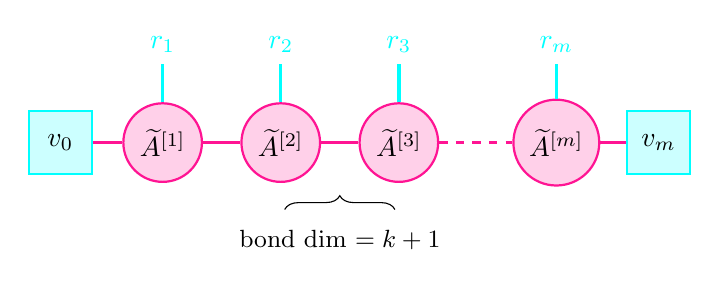
\begin{tikzpicture}[scale=1.0,
    site/.style={circle, draw=neonpink, fill=neonpink!20, minimum size=0.9cm, thick},
    boundary/.style={rectangle, draw=neonblue, fill=neonblue!20, minimum size=0.8cm, thick},
    bond/.style={very thick, neonpink},
    physical/.style={very thick, neonblue}]

% Boundary v_0
\node[boundary] (v0) at (-1.3, 0) {$v_0$};
% Site tensors
\node[site] (a1) at (0, 0)   {$\tA^{[1]}$};
\node[site] (a2) at (1.5, 0) {$\tA^{[2]}$};
\node[site] (a3) at (3.0, 0) {$\tA^{[3]}$};
\node[site] (am) at (5.0, 0) {$\tA^{[m]}$};
% Boundary v_m
\node[boundary] (vm) at (6.3, 0) {$v_m$};

% Bonds
\draw[bond] (v0) -- (a1);
\draw[bond] (a1) -- (a2);
\draw[bond] (a2) -- (a3);
\draw[bond, dashed] (a3) -- (am);
\draw[bond] (am) -- (vm);

% Physical indices
\draw[physical] (a1) -- ++(0,1) node[above] {$r_1$};
\draw[physical] (a2) -- ++(0,1) node[above] {$r_2$};
\draw[physical] (a3) -- ++(0,1) node[above] {$r_3$};
\draw[physical] (am) -- ++(0,1) node[above] {$r_m$};

% Bond dimension annotation -- brace sits well below the tensor circles
\draw[decorate, decoration={brace, amplitude=5pt}] 
   (1.55, -0.85) -- (2.95, -0.85) 
   node[midway, below=4pt] {\small bond dim $= k+1$};

\end{tikzpicture}
\end{center}

\bigskip
\begin{itemize}
    \item Compact representation of the \emph{coefficient tensor} $\alpha_r$.

    \medskip
    \item Each $\tA^{[j]}_{r_j}\in\C^{(k+1)\times(k+1)}$ is built from a
    single Gaussian binomial $\binom{\ell_j}{\ell_j-\ell_{j-1}}_{q_j}$.

    \medskip
    \item $\alpha_r = v_0\bigl(\prod_j \tA^{[j]}_{r_j}\bigr) v_m^{\top}$.
\end{itemize}
\end{frame}

%%

\begin{frame}{Why bond dimension $k+1$ matters}

\begin{itemize}
    \item Bond dimension $k+1$ is \emph{independent of $m$}.

    \bigskip
    \item Standard MPS preparation $\Rightarrow$ pilot state preparable
    in $\mathrm{poly}(m, k)$ gates.

    \bigskip
    \item For any polynomial $\calP(H)$ of degree $\le d$:
    \emph{same} site matrices, bond dim $d+1$ -- only the right boundary
    vector changes.

\end{itemize}
\end{frame}

%%

\begin{frame}{Exponential separation -- anticommuting Paulis}

\begin{itemize}
    \item Take $\{P_1,\ldots,P_m\}$ pairwise anticommuting (e.g.\ Majoranas).

    \medskip
    Then $\Omega$ is predecessor-uniform under \emph{any} ordering
    ($q_j = -1$).

    \bigskip
    \item Previous methods factor along connected components of the
    \emph{anticommutation graph} -- here the complete graph $K_m$.\;\;
    Cost: $\exp(m)$.

    \bigskip
    \item Our MPS: cost $O(mk^2)$ per amplitude.

    \medskip
    Concretely, $m=20$, $k=4$:\;\;$\sim 10^6$ vs.\ $\sim 320$.
\end{itemize}
\end{frame}

%%

\begin{frame}{Limitation -- predecessor-uniformity vs.\ locality}

\begin{itemize}
    \item In the Pauli case: if $P_j$ anticommutes with even one earlier
    generator, predecessor-uniformity forces $P_j$ to anticommute with
    \emph{all} earlier generators.

    \medskip
    $\Rightarrow$ $P_j$ shares support with \emph{every} earlier generator.

    \bigskip
    \item Tension with geometric locality: lattice generators with
    disjoint support always commute.

    \bigskip
    \item Predecessor-uniform Hamiltonians are \emph{highly non-local}.

    \medskip
    Mutually-anticommuting Majoranas are the prototype.
\end{itemize}
\end{frame}

%==========================================================
%  Closing
%==========================================================

\begin{frame}{Summary}

\begin{itemize}
    \item Introduced the \textbf{twisted multinomial coefficient}
    -- pair-dependent inversions.

    \bigskip
    \item Identified \textbf{predecessor-uniformity} as the structural
    condition that makes it factor into Gaussian binomials with
    \emph{site-dependent} parameters.

    \bigskip
    \item This gives an \textbf{exact MPS of bond dimension $k+1$} for
    HDQI pilot-state amplitudes -- exponentially better than previous
    methods on mutually-anticommuting families.

    \bigskip
    \item HDQI also requires efficient \emph{decoding}: finding
    Hamiltonians where both conditions hold simultaneously is the
    central open problem.
\end{itemize}
\end{frame}

%%

\begin{frame}{Open problems}

\begin{itemize}
    \item \textbf{Combinatorial side.} Complexity of evaluating
    $\binom{k}{k_1,\ldots,k_m}_\Omega$ for general (non-predecessor-uniform) $\Omega$?

    \bigskip
    \item \textbf{Quantum side.} Hamiltonians admitting both efficient
    pilot-state preparation \emph{and} efficient Hamiltonian-code decoding?

    \bigskip
    \item \textbf{Generalizations.} Block-structured analogues
    (predecessor-uniform within blocks) might lift the locality obstruction.
\end{itemize}
\end{frame}

%%

\begin{frame}{ありがとうございました}
\begin{center}
\begin{tikzpicture}[scale=0.95, background rectangle/.style={fill=spaceblack}, show background rectangle]

% Pin the picture bounds so the rotated Milky Way can't shift the slide
\useasboundingbox (-6, -2.8) rectangle (6, 4);

% Background stars
\foreach \i in {1,...,200} {
  \pgfmathsetmacro{\x}{rnd*12 - 6}
  \pgfmathsetmacro{\y}{rnd*4.0 - 0.5}
  \pgfmathsetmacro{\s}{0.008 + rnd*0.022}
  \pgfmathsetmacro{\op}{0.3 + rnd*0.6}
  \fill[white, opacity=\op] (\x,\y) circle (\s);
}

% Milky Way: drawn BEFORE the moon (and clipped) so the moon covers its center
\begin{scope}
  \clip (-6, -2.8) rectangle (6, 4);
  \begin{scope}
    \pgftransformrotate{25}
    \shade[inner color=neonpurple, outer color=spaceblack, opacity=0.35]
      (0, 1.5) ellipse (7.5 and 0.6);
    \shade[inner color=neonblue, outer color=spaceblack, opacity=0.25]
      (0, 1.5) ellipse (7.0 and 0.35);
  \end{scope}
  \begin{scope}
    \pgftransformrotate{25}
    \foreach \i in {1,...,400} {
      \pgfmathsetmacro{\x}{rnd*15 - 7.5}
      \pgfmathsetmacro{\yJitter}{(rnd-0.5)*1.0}
      \pgfmathsetmacro{\y}{1.5 + \yJitter}
      \pgfmathsetmacro{\s}{0.005 + rnd*0.018}
      \pgfmathsetmacro{\op}{0.3 + rnd*0.5}
      \fill[white, opacity=\op] (\x, \y) circle (\s);
    }
  \end{scope}
\end{scope}

% Moon halo glows
\fill[neonblue, opacity=0.10] (0, 1.2) circle (2.6);
\fill[neonblue, opacity=0.18] (0, 1.2) circle (2.0);

% Moon body: white center fading to neon blue at the edge
\shade[inner color=white, outer color=neonblue] (0, 1.2) circle (1.6);

% Moon craters
\fill[neonblue, opacity=0.45] (-0.45, 1.55) circle (0.18);
\fill[neonblue, opacity=0.35] (0.55, 0.95) circle (0.13);
\fill[neonblue, opacity=0.40] (0.25, 1.80) circle (0.10);
\fill[neonblue, opacity=0.45] (-0.65, 0.85) circle (0.15);
\fill[neonblue, opacity=0.30] (0.10, 1.35) circle (0.07);
\fill[neonblue, opacity=0.40] (-0.20, 0.70) circle (0.09);

% Synthwave grid
\synthwavegrid{-2.8}{2.0}

% Torii gate
\begin{scope}[shift={(0, -0.3)}, scale=1.0]
  \fill[toriired] (-1.20, -0.5) -- (-1.10, 1.7) -- (-0.95, 1.7) -- (-1.05, -0.5) -- cycle;
  \fill[toriired] (1.10, 1.7) -- (1.20, -0.5) -- (1.05, -0.5) -- (0.95, 1.7) -- cycle;
  \fill[toriired] (-1.10, 1.20) -- (1.10, 1.20) -- (1.10, 1.36) -- (-1.10, 1.36) -- cycle;
  \fill[toriired]
    (-1.45, 1.70) -- (1.45, 1.70)
    .. controls (1.55, 1.72) and (1.60, 1.78) .. (1.65, 1.85)
    -- (1.55, 1.95)
    -- (-1.55, 1.95)
    -- (-1.65, 1.85)
    .. controls (-1.60, 1.78) and (-1.55, 1.72) .. (-1.45, 1.70) -- cycle;
  \draw[neonyellow, line width=0.6pt, opacity=0.7] (-1.45, 1.92) -- (1.45, 1.92);
  \fill[toriired] (-0.06, 1.36) rectangle (0.06, 1.70);
\end{scope}

\node[neonyellow] at (0, 3.6) {\Large {\japanesefont ありがとうございました}};

\end{tikzpicture}
\end{center}
\end{frame}

\end{document}
